\documentclass{article}
\usepackage[utf8]{inputenc}

\usepackage{geometry}


\usepackage{graphicx}
\usepackage{pgfplots}
\usepackage{caption}

\usepackage[size=tiny, color=white]{todonotes}
\usepackage{float}
\usepackage{xypic}



\usepackage[T1]{fontenc}
%\usepackage{beramono}
\usepackage{listings}

\lstset{basicstyle=\ttfamily}

\setlength{\parindent}{0px}
\title{Adaptive Simulation Grids for Modern Simulation Software}
\author{Esther Koch (108016204757) and Leonid Ryvkin (108010206916)\\ ~\\ \textit{Supervised by Dennis Ogiermann und Maximilian Köhler}}
\date{February 2021}


\interfootnotelinepenalty=10000
\begin{document}

This code is the result of a project supervised by Dennis Ogiermann and Maximilian Köhler and carried out by Esther Koch and Leonid Ryvkin. 


\section{Goals of the project}
The goal of the project was to implement a subtype of the abstract type \texttt{JuAFEM.AbstractGrid} in a way enabling certain grid modifications (refinements and derefinements of cells). We worked against the following specification.\\

{\bf Design and constraints:}

\begin{itemize}
 \item A grid is a collection of cells (Elements) of a certain dimension $d$ in an $n$-dimensional euclidean space. 
 \item The cells can be convex quadrangles ($d=2$, $n=2$ or $n=3$) or convex hexahedra (cube-like elements, $d=n=3$).
 \item Cells are attached to each other along their faces.
 \end{itemize}
 

 {\bf Basic functionality:}
 
 \begin{itemize}
 \item In addition to all functionality of the JuAFEM grid (recovering vertices, edges, faces, cells, giving certain collections of these entities labels, etc.) it should be possible to refine/derefine cells.
 \item Refining a cell means subdividing it into several subcells (dividing a cell into 4 subcells for $d=2$, or 8 subcells for $d=3$). The refinements always happen along the centers of opposing sides, cf. Figure \ref{isotroicsplit}. 
 \begin{figure}[h!]
\centering
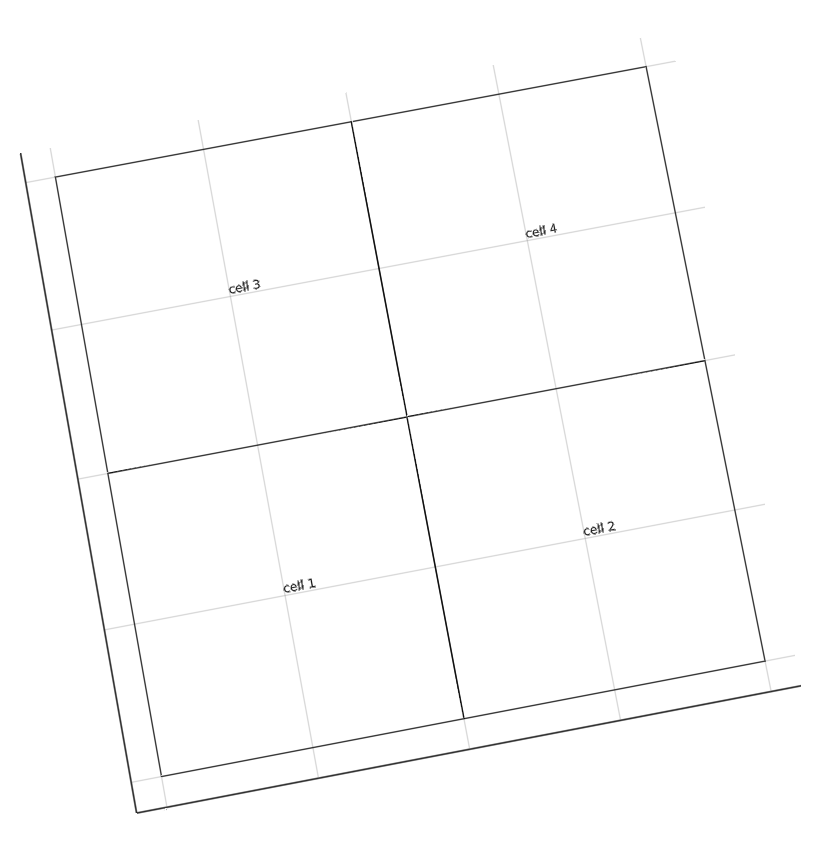
\includegraphics[width=0.3\textwidth]{images/2Dsplit.png}
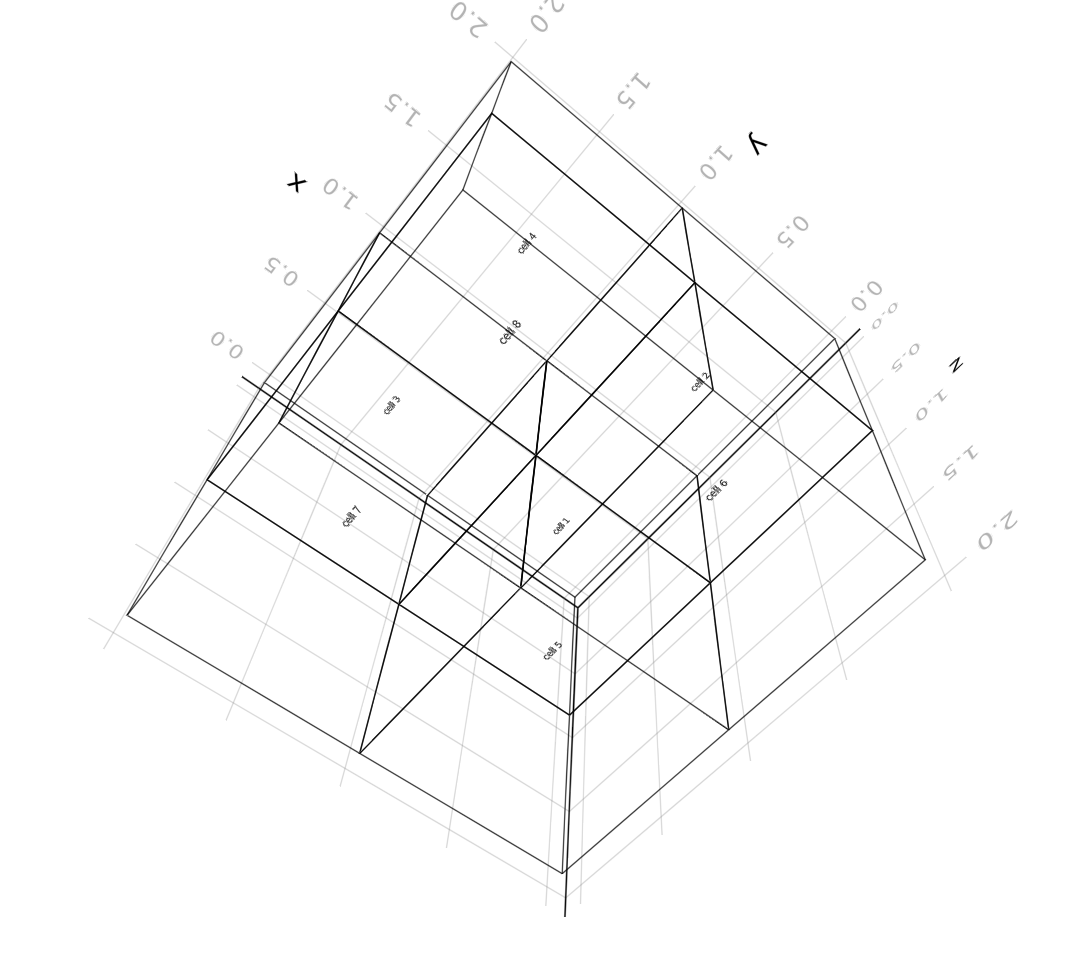
\includegraphics[width=0.4\textwidth]{images/3Dsplit.png}
\caption{isotropic split of 2D resp. 3D cell}\label{isotroicsplit}
\end{figure}
 \item Derefining simply reverts the refining operation.
 \item The biggest difficulty, if only one of two neighbouring cells is refined, then suddenly a big face is attached to several small ones. Some nodes turn up at the interior of cells and faces (i.e. are not on the corners). This information has to be recoverable from the grid in a way that JuAFEM can work with.
\end{itemize}



{\bf Stretch goals:}

\begin{itemize}
    \item Anisotropic splits: Splitting a cell into subcells might also be anisotropic, i.e. the split is carried out only along some axes. In $d=2$ an anisotropic split yields 2 subcells of a cell and for $d=3$ we get $2$ or $4$ subcells), cf. Figure \ref{anisotroicsplit}.
    \begin{figure}[h!]
\centering
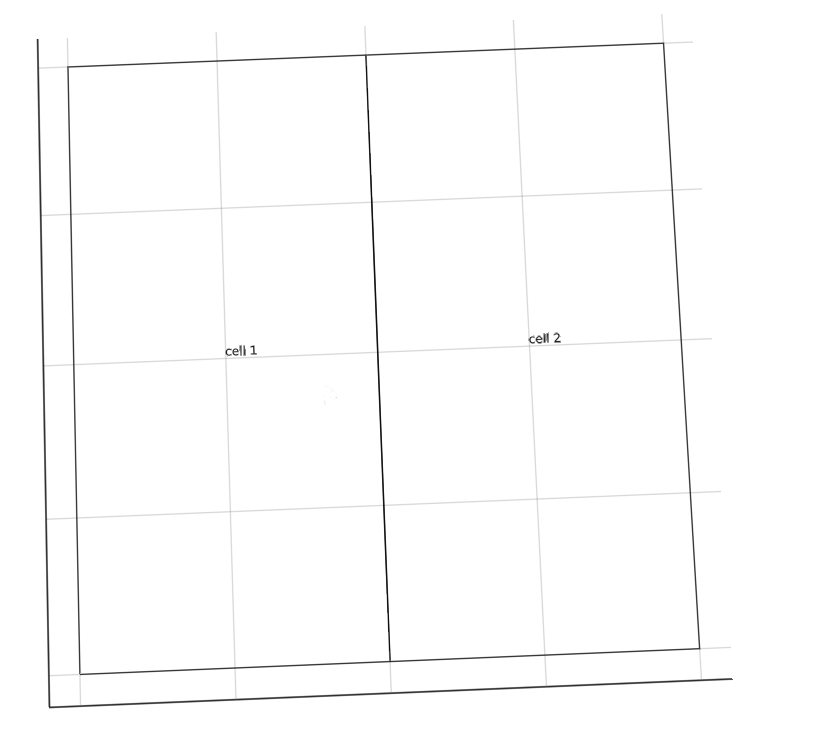
\includegraphics[width=0.3\textwidth]{images/2Dsplit-anisotropic.png}
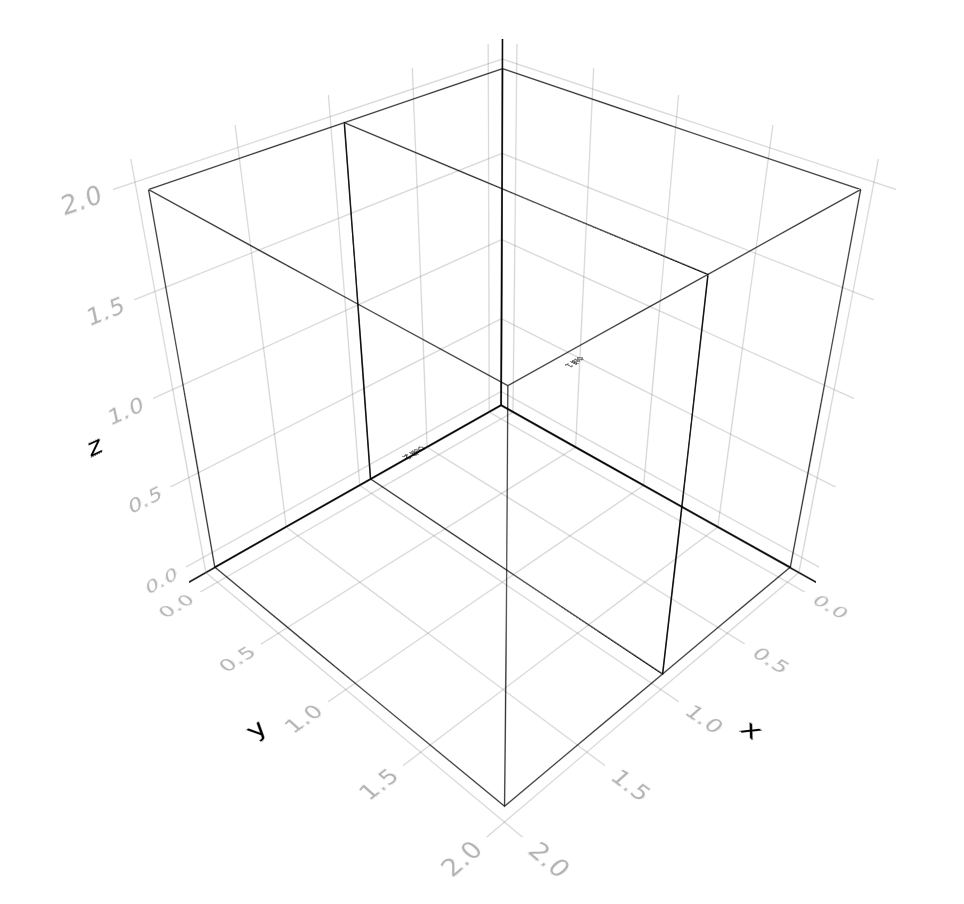
\includegraphics[width=0.3\textwidth]{images/3Dsplit-anisotropic-1.png}
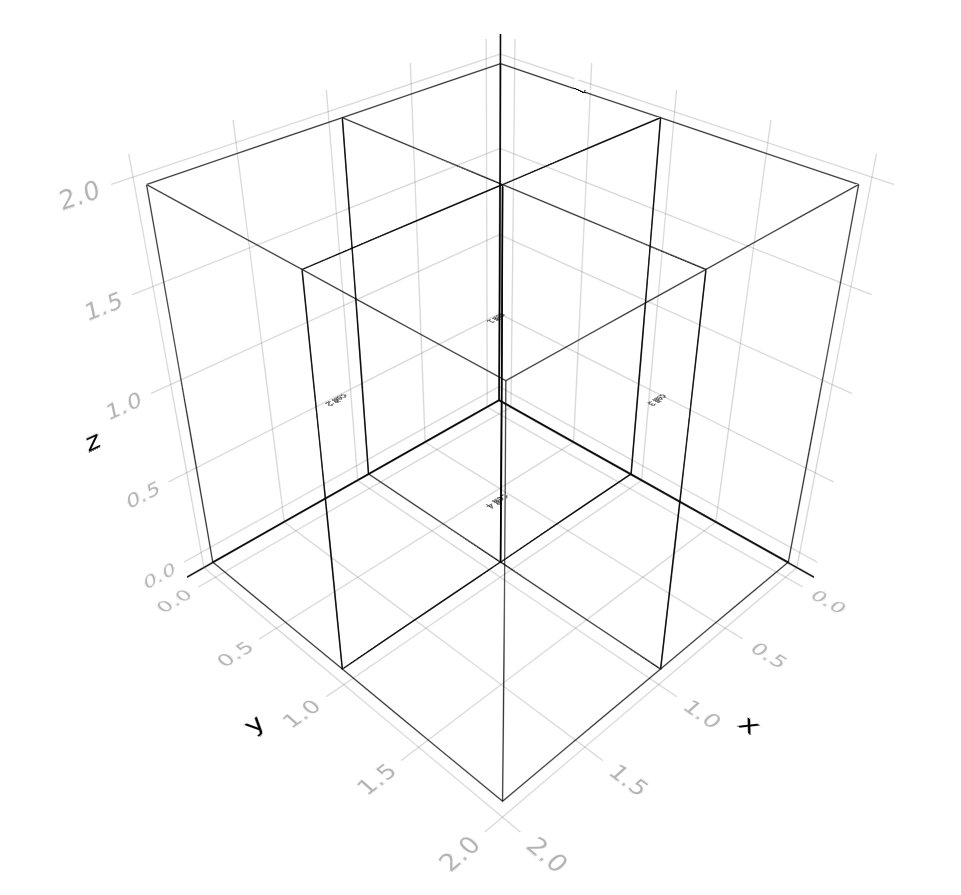
\includegraphics[width=0.3\textwidth]{images/3Dsplit-anisotropic-2.png}
\caption{The ways to anisotropically split 2D resp. 3D cell}\label{anisotroicsplit}
\end{figure}
    \item Non-manifold grids: In basic grids only two cells can be joined by a face. However, sometimes it is useful (especially for $d=2$) to allow for multi-cell joints, see e.g. Figure \ref{nonmf} 
     \begin{figure}[h!]
\centering
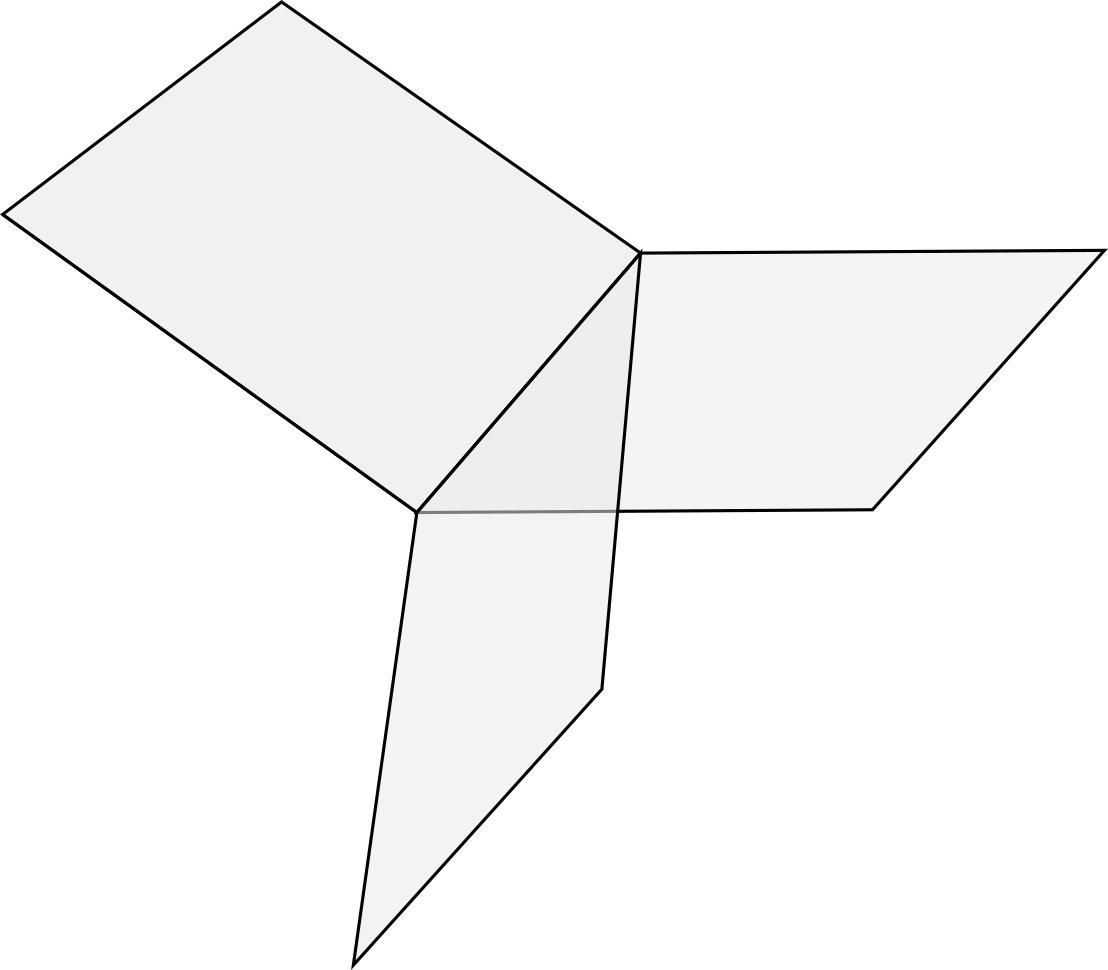
\includegraphics[width=0.4\textwidth]{images/non-manifold.png}
\caption{A non-manifold joint of three 2D-cells at one boundary in three dimensions.}\label{nonmf}
\end{figure}
    
    \item \textcolor{red}{Grids with varying cell dimension.}\footnote{Our realization does not exclude building such grids. However, the current refinement and derefinement functionality might not work properly close to the places where different dimensions meet.} 
\end{itemize}

\newpage
\section{Technical documentation}




\subsection{Introduction and Code structure} 
The module FEMRefinements.jl provides a realization of the \texttt{JuAFEM.AbstractGrid} type. The grid we construct is build from linear quadrilateral/ hexahedral  cells. Adjacent cells are connected through their boundaries. Cells, their boundaries, their boundaries boundaries etc. are all realized as instances of an \texttt{Element} struct, relizing the \texttt{JuAFEM.AbstractCell} type. In addition to basic \texttt{JuAFEM.grid} functionalities, our grid class \texttt{AdaptiveGrid} admits the refinement of cells (substituting a cell with a collection of smaller cells in a particular way). For the refinement procedure to be reversible, the old cells are not erased, but kept in the data structure. Hence, \texttt{Elements} store a lot of information: Relations between cells and subcells (boundaries and sub-boundaries), attachements to neighbouring cells, node locations. The core of our module are the structs \texttt{Element} and \texttt{AdaptiveGrid} together with the functions \texttt{refine!} and \texttt{derefine!}. The code is structured as follows:

\begin{itemize}
    \item {\bf src/FEMRefinements.jl:} This file mainly contains the imports, exports and and includes the actual code files. 
    \item {\bf src/elements.jl:} Contains the \texttt{Element} struct and its functions. In addition to reimplementing JuAFEM \texttt{Cell} methods (\texttt{Element} implements the abstract type \texttt{JuAFEM.AbstractCell}), also some methods for tree traversal are provided. Furthermore, some methods are provided to find out which nodes are on/in elements (mostly only working for boundary elements).
    \item {\bf src/refinements.jl:} This file contains the methods for refining and derefining cells. As these operations are local, no access to the grid is needed. The main subtleties are managing the masters of the faces and avoiding to create the same node twice (when a cell close to a subdivided cell is split, we want to reuse the same nodes for all new cells where possible).\footnote{For instance in the first step of the splitting procedure in Figure \ref{splitting-proc} five new nodes appear, and in the last step only 4, because the node on the center of the left hand side of the right cell already exists (it is the center of the righthand side of the left cell).}
    \item {\bf src/grid.jl:} Here the core struct \texttt{AdaptiveGrid} subtyping the \texttt{JuAFEM.AbstractGrid} type is implemented, along with its methods. Due to refinements and derefinements, nodes, faces and cells have no persistent integer number, however JuAFEM needs numbered lists as outputs, so most of the functions internally translate between the external linear numbering and the internal tree structure. The only parameter really necessary for the interior processing of the grid is \texttt{rootcells}, the other ones \texttt{cells, faces, nodes} are only stored, because they are accessed to often to be generated anew every time. The generation is carried out using the \texttt{update\_leafmesh!} function.
    \item {\bf src/utils.jl:} This file, written by M.K. and D.O. contains some functions necessary to use the grid with JuAFEM. 
    \item {\bf src/grid\_generators.jl:} Create a standard quadrilateral resp. hexahedral grid from two resp. 3 vectors. 
    \item {\bf src/visualization.jl:} A few grid and solution plotting methods, mostly for debugging. Written by M.K.
    \item {\bf test/runtests.jl} Tests for the \texttt{AdaptiveGrid} are provided. Contains an adaptation of most of the gridtests from JuAFEM and many additional tests for the refinement and derefinement interface.
    \item {\bf Examples/HeatEquation.jl} Adaptation of the HeatEquation example of JuAFEM with our AdaptiveGrid class, written by M.K. and D.O.
    \item {\bf Examples/HeatEquationMixed.jl} Further adaptation of the HeatEquation example of JuAFEM using a MixedDoFHandler, written by M.K. and D.O.
    \item {\bf Examples/helmholtz.jl} Adaptation of the Helmholtz example of JuAFEM to our grid class, written by M.K. and D.O.
\end{itemize}







\subsection{Design choices}
\begin{itemize}
    \item {\bf Cells:} A cell, realized by the struct \texttt{Element} is given by a list of its  \texttt{nodes} (corners, points in $n$-dimensional space)\footnote{In general there might be more nodes than corners (e.g. for quadratic instead of linear interpolation), however currently the package only supports linear elements}.  The order of the corners plays an important role and is fixed by the JuAFEM convention.
    \item {\bf Boundaries:} The cells are not connected directly, but through their boundaries. The boundaries are also instances of \texttt{Element}. Hence, any \texttt{Element} has parameters \texttt{boundaryof} and \texttt{boundaries}. For cells, the \texttt{boundaryof} parameter is set to \texttt{nothing}, for a boundary it points to the cell it is boundary of. For an element of dimension $d$, \texttt{boundaries} is an array of elements of dimension $d-1$, sorted by the JuAFEM convention. For 0-dimensional elements (given by one node) \texttt{boundaries} is left empty.  
    \item {\bf Tree structure:} For the bookkeeping of the refinements, a tree structure is chosen. When a cell is subdivided it stays in place and just gets the subcells as children. The tree-like structure relating the big cell and its subcells is saved in the \texttt{parent}, \texttt{children} parameters of \texttt{Element}. When a cell $c$ is split, the boundaries of the (appropriate) subcells $s_i$ are also linked to the boundaries of $c$ through their parent and children parameters. However, boundaries of boundaries are not connected via parent-children anymore for simplicity reasons.
    \item {\bf Attachments of boundaries:} The following approach is often utilized for adaptive grids\footnote{Zhao, Xinglin, et al. "Conformal and non-conformal adaptive mesh refinement with hierarchical array-based half-facet data structures." Procedia Engineering 124 (2015): 304-316.}: The boundaries of cells are called \emph{halffaces}. A face is made up of 1 halfface on one side (the master) and a set of halffaces spanning the same region on the other side.\footnote{This method does not allow two 2-dimensional boundaries in 3-dimensional space, of which one is split horizontally and the other vertically to be attached to each other.} To register, whether a halfface is the master \texttt{Element} has a \texttt{ismaster} boolean parameter, which is superfluous for non-cell-boundary elements. In order to allow for non-manifold structures, i.e. faces joining more than two sides, our faces contain one master and possibly several sets of slaves. Hence we will avoid the misleading notion of halffaces in the sequel. For an example of how master and slave halffaces behave, see Figure \ref{splitting-proc} below.
    As in our implementation of the grid, cells are not erased when they are split (cf. Tree structure), instead of pointing at a set of ``small boundaries'', we can point at their common ancestor. This is realized by the \texttt{attachedto} parameter of \texttt{Element}. It is a list of elements, which we only use for boundaries of cells (i.e. not for cells themselves and not for boundaries of boundaries of cells etc.). When a cell boundary is also a boundary of the grid, its \texttt{attachedto} is empty, when it is a slave, \texttt{attachedto} points only to its master and when it is a master \texttt{attachedto} points to all of its slaves. \textcolor{red}{The attachedto interface is only kept up to date for leaves of the tree, i.e. the boundaries that are not further subdivided, for a simpler code and better performance.}\footnote{Like in a tree, where only the few outer layers are actually alive, and the inside can has only supporting functions.}
    \item {\bf The actual grid} The core of the \texttt{AdaptiveGrid} struct is given by an array of its \texttt{rootcells}. All other data can be recovered through them by vertical traversal (parent to child) and horizontal traversal (cell to boundary to attachedto to boundaryof etc). 
    \item {\bf Refinement algorithm} The core of the package are the \texttt{refine!} (and derefine) functions. These functions call \texttt{split!} on a series of cells, and then execute \texttt{update\_leafmesh}. The \texttt{split!} method first creates the necessary new nodes, for splitting a given cell $c$. Then it checks the neighbourhood of the cell for whether some of these nodes already exist and removes the unnecessary new ones. Then the (up to 8) subcells $s_i$ of $c$ are created and attached to one another. The last and most subtle step is gluing the $s_i$ into the grid, along the boundaries of $c$. This is delegated to \texttt{attach\_children!}. \texttt{attach\_children!} has three options: either the boundary of $c$ is a slave (very simple case), or it can be made a slave (using \texttt{make\_master!} on another boundary it is attached to, simple case) or the master has to be split, in which case the slaves have to be distributed correctly among the subboundaries of the master.
    \item {\bf Derefinement algorithm} works analogously calls \texttt{derefine!} on an individual cell $c$, where the only subtlety is gluing the boundary of $c$ back into the grid, which is realized by the \texttt{unattach\_children} function.
\end{itemize}


\begin{figure}[h!]
\centering
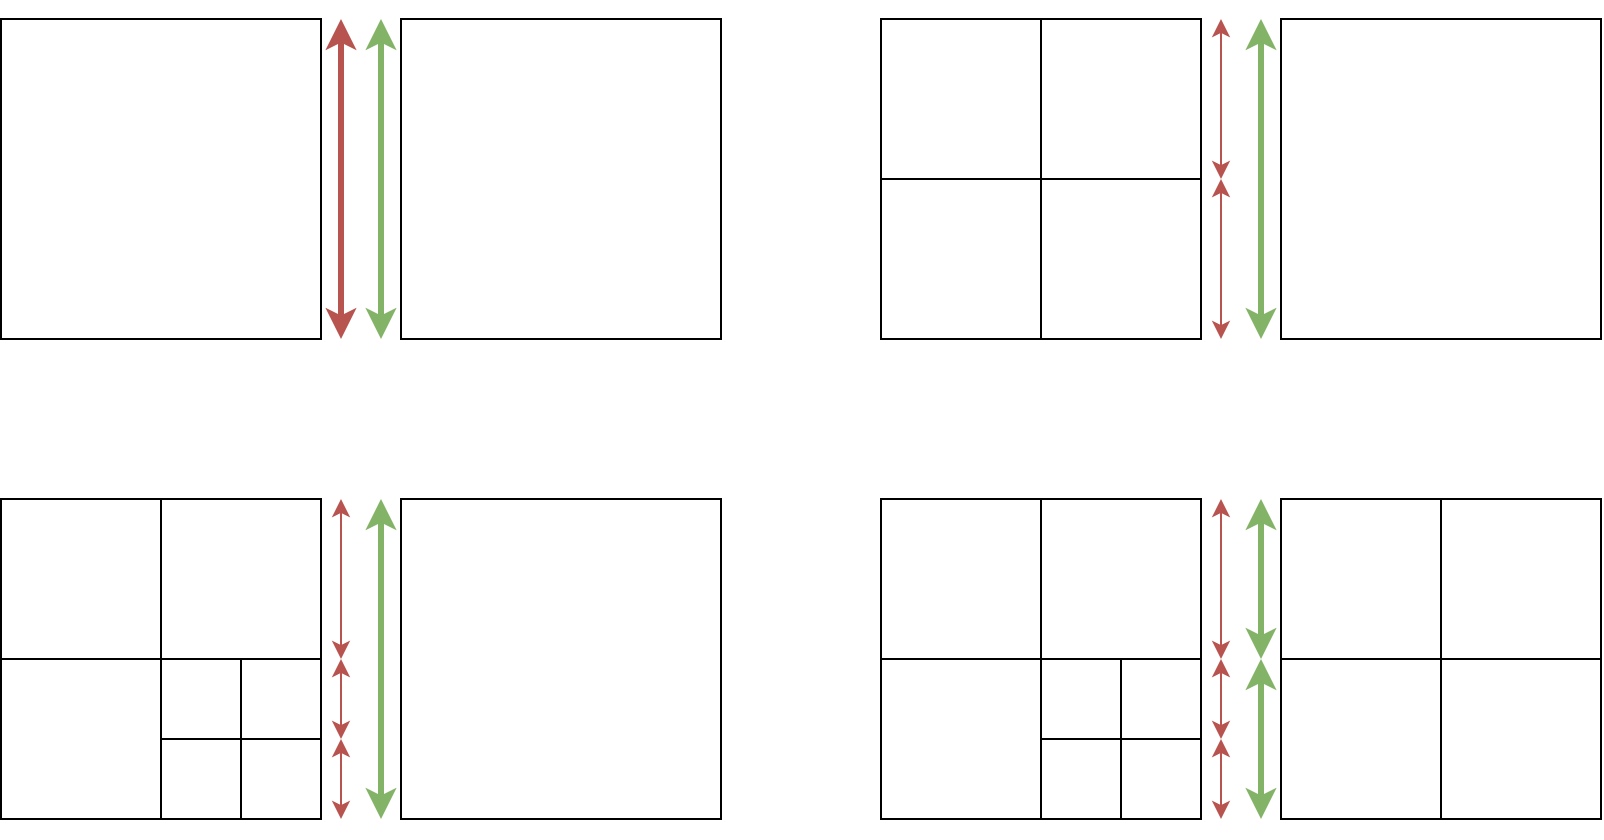
\includegraphics[width=0.8\textwidth]{images/splitting-procedure.png}
\caption{The development of master-slave relationships for two neighbouring cells, masters are \textcolor{green}{green} and slaves are \textcolor{red}{red}. In the first picture there is one face (one master attached to one slave). Then the left cell is split, and we have a master attached to two slaves (still one face). After a further split, the master has three slaves (still one face). Finally the right cell, and hence the master splits, now we have two masters, one with one slave and one with two (Now we have 2 faces). Note that in the last image the top master and slave could be interchanged.}\label{splitting-proc}
\end{figure}
\newpage



\subsection{Costs of the functions}

In the runtime expectations described below, we assume $n$ to be the number of original cells and $d$ be the maximal depth or refinement. We further assume that the number of non-manifold-joints (i.e. the number of places where more than two boundaries are joined) is not significant. Especially, the space required by a grid can go up to $\mathcal O(8^d\cdot n)$. We omit methods with constant runtime. Most methods in the element.jl and refinements.jl files operate locally and don't depend on $n$ directly:\footnote{The only exception is \texttt{eltocell}, which needs to go through the whole $\mathcal{O}(8^d \cdot n)$ long nodelist, to return the indices of the corners of the element}
\begin{itemize}
    \item {\bf Methods with depth-linear runtime  $\mathcal O(d)$} Mostly due to (simple) tree traversal
    \begin{itemize}
        \item \texttt{ultimate\_ancestor}
        \item \texttt{findlowestancestorwithnodes}
        \item \texttt{descent\_until\_split}
        \item \texttt{getdepth}
    \end{itemize}
    \item {\bf Methods with depth-exponential runtime $\mathcal O(8^d)$ } (3D case), mostly due to tree traversal with branching (i.e. doing something for all children)
        \begin{itemize}
        \item \texttt{collect\_children}
        \item \texttt{getcontainednodes}, \texttt{getinteriornodes}, \texttt{getneighbourhood}, \texttt{getnodeneighborhood}
        \item \texttt{have\_identical\_leaves}
        \item \texttt{make\_master!} (as a big boundary can be connected to many small ones)
        \item \texttt{attach\_children!}, \texttt{unattach\_children!} and hence \texttt{derefine!}.
        \item \texttt{split!} and \texttt{isotropic\_split!}, mostly due to checking, whether the necessary new nodes are already in the grid. More specifically getting the \texttt{nodeneighbourhood} and applying \texttt{substitute\_nodes!} are the costly part.
        \end{itemize}
\end{itemize}

On the other hand, methods in grid.jl, typically have to find indices of elements in a list (node, cell, face etc.) and thus have runtimes of at least $\mathcal O(n\cdot 8^d)$ i.e. linear in the total number of nodes (or cells). Especially, the method \texttt{update\_leafmesh!} and hence \texttt{refine!} and \texttt{derefine!} have this runtime.




\subsection{Basic use}

\begin{lstlisting}
using FEMRefinements #our module
using JuAFEM #appropriate version necessary, enabling use of external grids
import Makie # just for plotting 

#define 3 vectors
v1 = Vec((2.0, 0.0, 0.0))
v2 = Vec((0.0, 2.0, 0.0))
v3 = Vec((0.0, 0.0, 2.0))

#generate a grid
grid = generate_grid3D(2, 2, 2, v1, v2, v3);

#refine all cells isotropically
FEMRefinements.refine!(grid, collect(1:getncells(grid)))

#refine one cell anisotropically along the first axis
FEMRefinements.refine!(grid, [1], [[1]])

#get nonconformal information (i.e. information about hanging nodes)
ncinfo = getncinfo(grid)

# plot the grid
Makie.mesh(grid)
\end{lstlisting}
The output of the above plot can be seen in Figure \ref{basicex}.

\begin{figure}[h!]
\centering
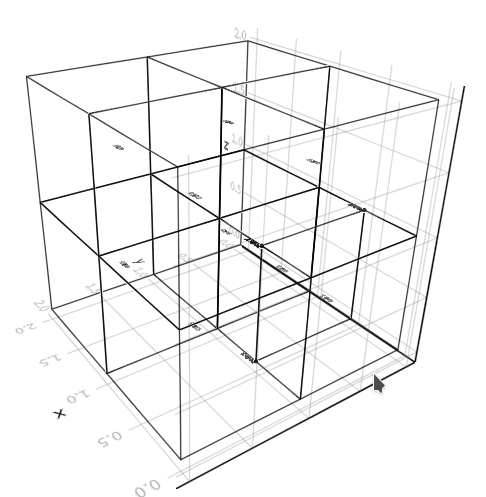
\includegraphics[width=0.3\textwidth]{images/example-3d-grid.png}\\
\caption{Plot of the 3D-grid generated and refined above}
\label{basicex}
\end{figure}


\newpage
\subsection{State of the code, future work}

\begin{itemize}
    \item \textcolor{black}{Tested to some extend:} 
    \begin{itemize}
        \item quadrilateral 2-dimensional grids in 2 and 3 dimensions.
        \item  hexahedral 3-dimensional grids.
        \item refinement (isotropically or anisotropically) and derefinement. 
        \item output in a JuAFEM compatible way.
        \item information on hanging nodes, i.e. nodes that are not on the corners of master-boundaries (= faces).
    \end{itemize}
    
    \item \textcolor{black}{Implemented, untested:} 
    \begin{itemize}
    \item The possibility to have grids with more complex topology (tori, rings, spheres etc).
        \item Non-manifold grids (with more than two sides touching).
    \end{itemize}
    \item \textcolor{black}{partially implemented/unimplemented:}
    \begin{itemize}\item 1-dimensional grids (easy to add). \item Grids of mixed dimension (Here some change in JuAFEM would be necessary, splitting near the dimension jumps could be difficult).\item  Higher dimensions (Currently not possible due to limitations of Tensors.jl. Implementation changes could be necessary for finding node-neighbourhoods of elements and checking whether a node is in an element, where the linear algebra is currently not dimension-agnostic).
\end{itemize}
\item \textcolor{black}{Possible problems:}
    \begin{itemize}
        \item Currently the way to check whether a certain node is already in the grid is by checking coordinates, this is not precise and might lead to problems at very refined (small) cells. Similarly, the checks of whether a node is in a cell are numerical calculations and not algebraic and thus could also break due to machine precision problems.
        \item To improve performance, currently when an new node candidate is added to the grid, not all existing nodes are checked, when trying to find whether it already exists, but only a node-neighborhood of the cell. The generation of this neighbourhood could be unreliable.  \footnote{This is rather a 3D than a 2D problem and could be mitigated by also attaching edges etc. to each other and not only faces. However that could harm performance and needs some coding work.}
        \item The management of which boundaries are masters and how they are attached to each other is quite fiddly.Problems in reassigning the master can easily occur, especially when having non-manifold meshes in 3 dimensions. 
        \item We do not follow the JuAFEM convention for ordering edges of a 3-dimensional cell, because for us they are just boundaries of boundaries. \footnote{If needed, this can be easily changed.}
    \end{itemize}

\item \textcolor{black}{Potential improvements:}
    \begin{itemize}
        \item More dimension-agnostic approach, especially for the refinement parts.
        \item Algebraic instead of numeric way of finding nodes nearby.
        \item performance improvements e.g. by not having edges (and 0-dimensional elements!) as separate entities. Use of static data structures instead of Arrays. Different data structures for different types of element to avoid unnecessary field. 
        \item A grid construction toolkit, (where one can, for example, glue grids to one another along elements) could be quite useful.
        \item Instead of throwing an error when \texttt{refine!}is called on a set of cells where some cells can not be refined, the refinement procedure should just throw a warning and refine wherever possible.
        \item Most methods in grid.jl have a very bad runtime, as the indices of elements and nodes have to be retrieved from very long lists. This could be improved by appropriately saving the indices directly in the cells or buffering them.
    \end{itemize}



\end{itemize}


\end{document}


